\documentclass{article}
\usepackage[top=1in, bottom=1in, left=1in, right=1in]{geometry}
\usepackage{graphicx}
\begin{document}

\begin{flushright}
Matt Jibson \\
EG 520 \\
HW 2
\end{flushright}

\begin{itemize}
	\item[7.2]
		\begin{itemize}
			\item[a.] \ \\ 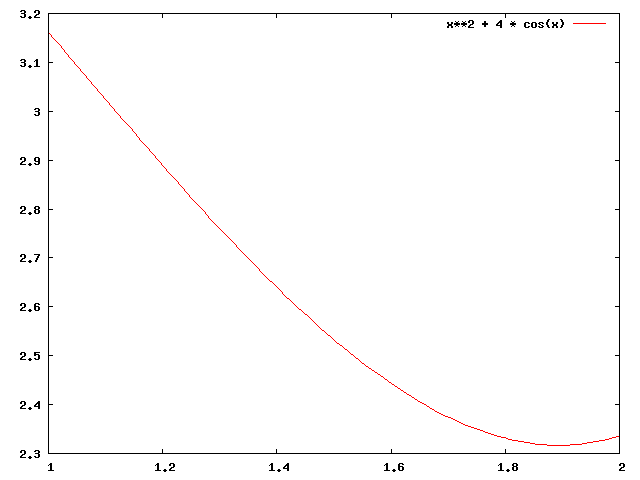
\includegraphics[width=0.5\linewidth]{72a.png}
			\item[b.] $(0.61803)^N \le 0.2/1 \Rightarrow N = 4$. \\
				\begin{tabular}{cccccc}
					\hline
					Iteration $k$ & $a_k$ & $b_k$ & $f(a_k)$ & $f(b_k)$ & New uncertainty interval \\
					\hline
					1 & 1.3820 & 1.6180 & 2.6607 & 2.4292 & [1.3820, 2.0000] \\
					2 & 1.6180 & 1.7639 & 2.4292 & 2.3437 & [1.6180, 2.0000] \\
					3 & 1.7639 & 1.8541 & 2.3437 & 2.3196 & [1.7639, 2.0000] \\
					4 & 1.8541 & 1.9098 & 2.3196 & 2.3171 & [1.8541, 2.0000] \\
					\hline
				\end{tabular}
			\item[c.] $F_{N + 1} \ge \frac{1 + 2 \epsilon}{0.2} \Rightarrow N = 4$. \\
				\begin{tabular}{ccccccc}
					\hline
					Iteration $k$ & $p_k$ & $a_k$ & $b_k$ & $f(a_k)$ & $f(b_k)$ & New uncertainty interval \\
					\hline
					1 & 0.3750 & 1.3750 & 1.6250 & 2.6688 & 2.4239 & [1.3750, 2.0000] \\
					2 & 0.4000 & 1.6250 & 1.7500 & 2.4239 & 2.3495 & [1.6250, 2.0000] \\
					3 & 0.3333 & 1.7500 & 1.8750 & 2.3495 & 2.3175 & [1.7500, 2.0000] \\
					4 & 0.5000 & 1.8750 & 1.8625 & 2.3175 & 2.3186 & [1.7500, 1.8625] \\
					\hline
				\end{tabular} \\
				The numbers found in the above tables were computed using a program authored by me as implementations of the two methods.
		\end{itemize}
	\item[8.1]
	\item[8.3] $u_k = r (1 - \rho)^k, r = \textrm{range}, \rho = \frac{3 - \sqrt{5}}{2} \Rightarrow \frac{r (1 - \rho)^{(k + 1)}}{(r (1 - \rho)^{(k)})^p} = \frac{r}{r^p} (1 - \rho)^{k + 1 - kp} = r^{(1 - p)} (1 - \rho)^{k(1 - p) + 1}$, hence the order of convergence is 1 since for $p < 1$ the sequence converges to 0 and if $p > 1$ it converges to $\infty$.
	\item[8.13]
	\item[8.17]
	\item[9.1]
		\begin{itemize}
			\item[a.] $g(x) = \nabla f(x^{(k)}) = 4 (x - x_0)^3, F(x) = 12 (x - x_0)^2, F(x)^{-1} = \frac{1}{12 (x - x_0)^2}, x^{(k + 1)} = x^{(k)} - F(x^{(k)})^{-1} g^{(k)} = x^{(k)} - \frac{1}{12 (x - x_0)^2} 4 (x^{(k)} - x_0)^3 = x^{(k)} - \frac{1}{3} (x^{(k)} - x_0)$
			\item[b.] $y^{(k+1)} = |x^{(k+1)} - x_0| = |x^{(k)} - \frac{1}{3} (x^{(k)} - x_0) - x_0| = |\frac{2}{3} x^{(k)} - \frac{2}{3} x_0| = \frac{2}{3}|x^{(k)} - x_0| = \frac{2}{3} y^{(k)}$
			\item[c.] For any $x_0$, the shape of the function is always U-like, with one solution at $f(x) = 0$, and all other values $> 0$. A change in $x_0$ only shifts the function left or right. Hence, the next term will always point in the direction of $x_0$.
			\item[d.] $\frac{|x^{(k + 1)}|}{|x^{(k)}|^p} = \frac{|\frac{2}{3} y^{(k)}|}{|y^{(k)}|^p} = \frac{2}{3} y^{k(1 - p)}$. If $p < 1$, the sequence converges to 0, if $p > 1$, the sequence converges to $\infty$, hence the order of convergence is 1.
			\item[e.] There is no $x^*$ such that $\nabla f(x^*) = 0$, hence the theorem does not hold.
		\end{itemize}
	\item[9.3]
		\begin{itemize}
			\item[a.] At $[1, 1]^T, f(x) = 0$. And, since both terms where $x_1$ and $x_2$ are used are squared and hence positive, and the only remaining operations are multiplation and addition of positive numbers, there is no way for the function to return a value $< 0$. Hence, $[1, 1]^T$ is the unique global minimizer.
			\item[b.] $f(x) = 100(x_2 - x_1^2)^2 + (1 - x_1)^2, \nabla f(x^k) = [-400(x_2 - x_1^2)x_1 - 2(1-x_1), 200(x_2 - x_1^2)]^T$,
			\begin{displaymath}
			F(x) = \left[ \begin{array}{cc}
				1200 x_1^2 - 400 x_2 + 2 & -400 x_1 \\
				x_1 - 400 & 200
			\end{array} \right],
			\end{displaymath}
			\begin{displaymath}
			F(x)^{-1} = \frac{1}{(1200 x_1^2 - 400 x_2 + 2) (200) - (-400 x_1) (x_1 - 400)} \left[ \begin{array}{cc}
				200 & 400 x_1 \\
				-x_1 + 400 & 1200 x_1^2 - 400 x_2 + 2
			\end{array} \right]
			\end{displaymath}
			Iter 1: $g^{(0)} = [-2, 0], F(x^{(0)})^{-1} = [[0.5, 0], [1, 0.005]], x^{(1)} = [1, 2]$ \\
			Iter 2: $g^{(1)} = [-400, 200], F(x^{(1)})^{-1} = [[-0.0025, -0.00505], [-0.00504, -0.005075]], x^{(2)} = [1, 1]$
			\item[c.] Iter 1: $g^{(0)} = [-2, 0], x^{(1)} = [0.1, 0]$ \\
				Iter 2: $g^{(1)} = [-1.4, -2], x^{(2)} = [0.17, 0.1]$ \\
		\end{itemize}
\end{itemize}

\end{document}